\chapter{Os plásticos e os materiais sintéticos}\label{ch:g8:plastics}

Conte os objetos de \omterm{def:g8:plastics:plastic}{plástico} em que você toca numa só manhã: uma escova
de dentes, uma garrafa, uma capa de chuva, uma capinha de celular, o
banco de um ônibus, a sacola das compras. Quase nenhum deles existia há
cento e vinte anos, e nenhum cresceu numa árvore ou foi tirado do chão.
Os \omterm{def:g8:plastics:plastic}{plásticos} são materiais inventados pelos químicos --- leves, baratos,
impermeáveis, moldáveis em qualquer forma --- e esse próprio sucesso
virou um problema.

\begin{recall}
Os \omterm{def:g5:raw-materials-and-recycling:natural-material}{materiais naturais} são usados mais ou menos como são encontrados na
natureza; os \omterm{def:g5:raw-materials-and-recycling:natural-material}{materiais fabricados} são produzidos a partir de
matérias-primas transformadas, e a \omterm{def:g5:raw-materials-and-recycling:recycling}{reciclagem} transforma o material de
objetos velhos em objetos novos
(\cref{ch:g5:raw-materials-and-recycling}). A \omterm{def:g4:what-a-fire-needs:burning}{combustão} de um
\omterm{def:g4:what-a-fire-needs:fuel}{combustível} feito de carbono e hidrogênio dá dióxido de carbono e água
(\cref{ch:g8:combustion-and-fuels}).
\end{recall}

\begin{omfigure}
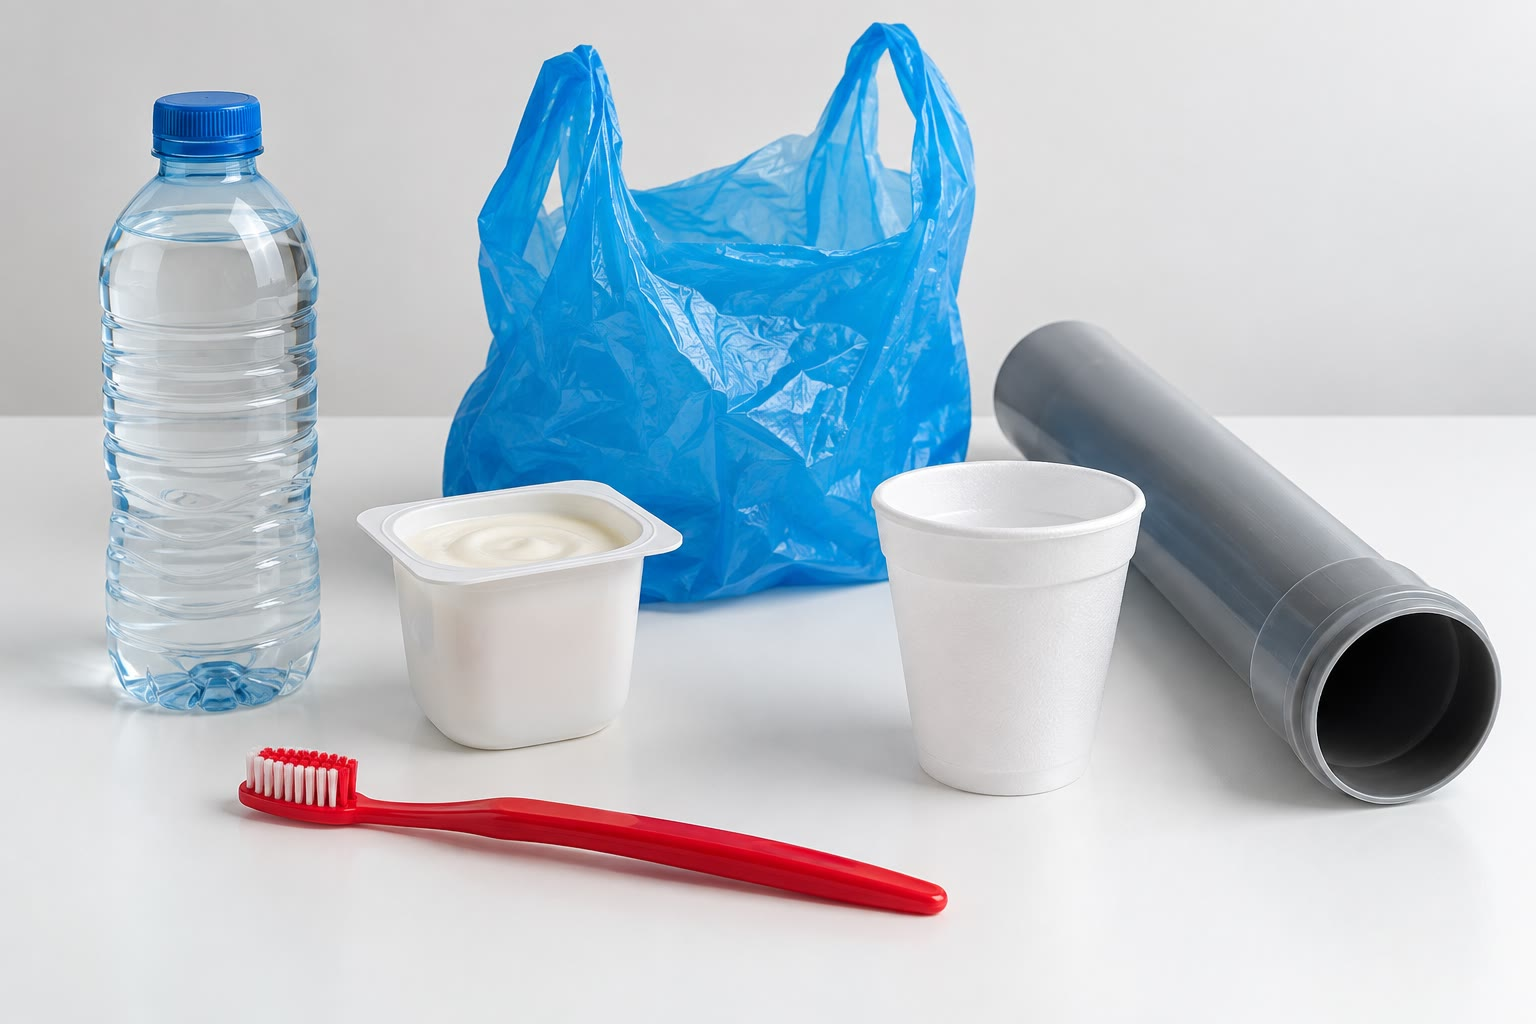
\includegraphics[width=0.55\linewidth]{images/book1/ai/g8-plastic-objects.jpg}

{\small Objetos de \omterm{def:g8:plastics:plastic}{plástico} do dia a dia: uma garrafa, um pote, uma
sacola, um cano, um copo, uma escova de dentes.}
\end{omfigure}

\section{Materiais naturais, artificiais e sintéticos}

\begin{definition}[Materiais artificiais e sintéticos]\label{def:g8:plastics:artificial}
Entre os \omterm{def:g5:raw-materials-and-recycling:natural-material}{materiais fabricados}, um \emph{material
artificial}\index{material artificial} é produzido transformando
quimicamente um \omterm{def:g5:raw-materials-and-recycling:natural-material}{material natural}: o papel e a viscose (um tecido), a
partir da celulose da madeira. Um \emph{material
sintético}\index{material sintetico@material sintético} é produzido a partir de substâncias
construídas pelos químicos, na maioria das vezes a partir do petróleo, e
não tem equivalente natural: o náilon, o poliéster, os \omterm{def:g8:plastics:plastic}{plásticos}.
\end{definition}

\begin{omfigure}
\begin{tikzpicture}[font=\small, level distance=1.5cm,
    box/.style={draw=omDef, fill=omDef!6, rounded corners=2pt, align=center,
      inner sep=4pt, text width=3.3cm},
    level 1/.style={sibling distance=6.4cm},
    level 2/.style={sibling distance=3.8cm},
    edge from parent/.style={draw, thick, omDef, ->}]
  \node[box] {materiais}
    child {node[box] {naturais\\ \footnotesize algodão, lã, madeira}}
    child {node[box] {fabricados}
      child {node[box] {artificiais\\ \footnotesize papel, viscose}}
      child {node[box, draw=omProp, fill=omProp!6] {sintéticos\\ \footnotesize náilon,
        poliéster, plásticos}}};
\end{tikzpicture}

{\small \omterm{def:g5:raw-materials-and-recycling:natural-material}{Materiais naturais}, artificiais e sintéticos.}
\end{omfigure}

\section{O que são os plásticos}

\begin{definition}[Plástico]\label{def:g8:plastics:plastic}
Um \emph{plástico}\index{plastico@plástico} é um \omterm{def:g8:plastics:artificial}{material sintético} formado por
\omterm{def:g7:atoms-and-molecules:molecule}{moléculas} muito longas, que pode ser moldado --- na maioria das vezes
quando está quente e mole --- e conserva a forma depois de esfriar. A
maioria dos plásticos é produzida a partir do petróleo ou do gás natural.
\end{definition}

\begin{remark}[Moléculas muito longas]\label{rem:g8:plastics:long}
Uma \omterm{def:g7:atoms-and-molecules:molecule}{molécula} de água contém três \omterm{def:g7:atoms-and-molecules:atom}{átomos}; uma \omterm{def:g7:atoms-and-molecules:molecule}{molécula} de um \omterm{def:g8:plastics:plastic}{plástico} pode
conter dezenas de milhares deles, ligados numa longa cadeia, como um
colar de contas idênticas. Como essas cadeias são construídas é o
assunto de um capítulo no fim deste livro.
\end{remark}

\begin{omfigure}
\begin{tikzpicture}[font=\small]
  \foreach \k in {0,...,17} {
    \pgfmathsetmacro\x{0.62*\k}
    \pgfmathsetmacro\y{0.35*sin(40*\k)}
    \shade[ball color=omDef!50] (\x,\y) circle (0.22);
  }
  \node[anchor=west] at (11.2,0) {\dots};
  \node[anchor=north, align=center] at (5.3,-0.6) {uma cadeia de milhares de unidades idênticas};
\end{tikzpicture}

{\small Uma imagem, não um modelo: a \omterm{def:g7:atoms-and-molecules:molecule}{molécula} de um \omterm{def:g8:plastics:plastic}{plástico} é uma cadeia
muito longa de unidades idênticas.}
\end{omfigure}

\begin{history}[A baquelite, 1907]
O primeiro \omterm{def:g8:plastics:plastic}{plástico} totalmente sintético foi produzido pelo químico Leo
Baekeland em 1907, a partir do fenol, obtido do alcatrão de hulha, e do
formaldeído. A baquelite, dura, escura e resistente ao calor, virou o
material dos telefones, dos rádios e dos interruptores elétricos. O
náilon veio na década de 1930, e depois os \omterm{def:g8:plastics:plastic}{plásticos} das garrafas e das
sacolas, após a Segunda Guerra Mundial.
\end{history}

\begin{omfigure}
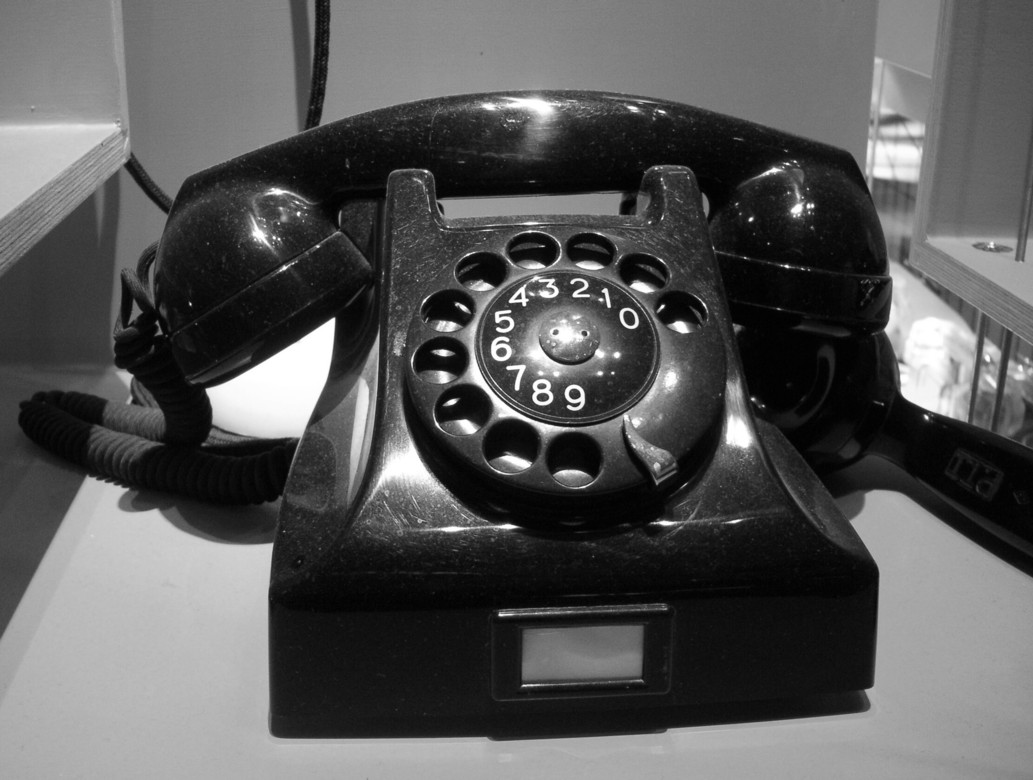
\includegraphics[width=0.42\linewidth]{images/book1/bakelite-telephone.jpg}

{\small Um telefone de baquelite de 1947. Foto: Holger Ellgaard,
CC BY-SA 3.0.}
\end{omfigure}

\section{Os principais plásticos e os seus códigos}

\begin{definition}[Código de identificação de resinas]\label{def:g8:plastics:code}
O \emph{código de identificação de resinas}\index{codigo de identificacao de resinas@código de identificação de resinas}
é um número de 1 a 7, impresso dentro de um
triângulo de setas num objeto de \omterm{def:g8:plastics:plastic}{plástico}, que dá o nome do \omterm{def:g8:plastics:plastic}{plástico} de
que ele é feito, para que o objeto possa ser separado para a
\omterm{def:g5:raw-materials-and-recycling:recycling}{reciclagem}. O triângulo não quer dizer que o objeto vai ser reciclado.
\end{definition}

\begin{proposition}[Sete códigos]\label{prop:g8:plastics:codes}
Os códigos, com os usos mais comuns de cada \omterm{def:g8:plastics:plastic}{plástico}:
\begin{center}
\small
\begin{tabular}{cll}
\hline
código & \omterm{def:g8:plastics:plastic}{plástico} & objetos típicos \\
\hline
1 & PET, poli(tereftalato de etileno) & garrafas de água e de refrigerante, fibras de fleece \\
2 & PEAD, polietileno de alta densidade & frascos de leite e de xampu, tampas \\
3 & PVC, poli(cloreto de vinila) & canos, esquadrias de janelas, cabos \\
4 & PEBD, polietileno de baixa densidade & sacolas, filmes \\
5 & PP, polipropileno & potes de iogurte, tampinhas, para-choques \\
6 & PS, poliestireno & copos e bandejas de isopor, caixas de CD \\
7 & outros \omterm{def:g8:plastics:plastic}{plásticos} & \omterm{def:g6:pure-substances-and-mixtures:mixture}{misturas}, embalagens multicamadas \\
\hline
\end{tabular}
\end{center}
\end{proposition}

\begin{omfigure}
\begin{tikzpicture}[font=\small]
  \foreach \n/\lab in {1/PET, 2/PEAD, 3/PVC, 4/PEBD, 5/PP, 6/PS, 7/OUTROS} {
    \begin{scope}[xshift=(\n-1)*2.1cm]
      \foreach \a in {90,210,330} {
        \pgfmathsetmacro\b{\a+120}
        \draw[omDef, line width=1.1pt, ->, >={Stealth[length=4pt]}]
          ($(\a:0.75)!0.14!(\b:0.75)$) -- ($(\a:0.75)!0.86!(\b:0.75)$);
      }
      \node[font=\bfseries] at (0,-0.05) {\n};
      \node[anchor=north, font=\footnotesize] at (0,-0.8) {\lab};
    \end{scope}
  }
\end{tikzpicture}

{\small Os sete \omterm{def:g8:plastics:code}{códigos de identificação de resinas}, cada um com a
sigla do seu \omterm{def:g8:plastics:plastic}{plástico}.}
\end{omfigure}

\section{Termoplásticos e termofixos}

\begin{definition}[Termoplástico e termofixo]\label{def:g8:plastics:thermoplastic}
Um \emph{termoplástico}\index{termoplastico@termoplástico} amolece cada vez que é
aquecido e endurece de novo quando esfria: ele pode ser derretido e
moldado muitas e muitas vezes (PET, polietileno, PVC, polipropileno,
poliestireno). Um \emph{termofixo}\index{termofixo} endurece para sempre
quando é aquecido e moldado pela primeira vez: aquecido de novo, ele não
amolece, mas carboniza (a baquelite, as resinas das colas e dos cascos
de barcos).
\end{definition}

\begin{remark}[Quais podem ser reciclados]\label{rem:g8:plastics:which}
Os \omterm{def:g8:plastics:thermoplastic}{termoplásticos} podem ser derretidos e moldados de novo: são eles os
\omterm{def:g8:plastics:plastic}{plásticos} reciclados em objetos novos. Os \omterm{def:g8:plastics:thermoplastic}{termofixos} não podem ser
derretidos de novo.
\end{remark}

\section{Os plásticos no meio ambiente}

\begin{proposition}[Os plásticos duram]\label{prop:g8:plastics:last}
% ledger: plastics:use-2019, plastics:waste-2019, plastics:recycled-share-2019
O mundo usou cerca de 460 milhões de toneladas de \omterm{def:g8:plastics:plastic}{plásticos} em 2019 e
jogou fora cerca de 353 milhões de toneladas de lixo \omterm{def:g8:plastics:plastic}{plástico}; o
\omterm{def:g8:plastics:plastic}{plástico} reciclado correspondeu a só cerca de \qty{6}{\percent} do
\omterm{def:g8:plastics:plastic}{plástico} usado. Os \omterm{def:g8:plastics:plastic}{plásticos} não apodrecem: na natureza, eles se
quebram em pedaços cada vez menores, os microplásticos, que são
encontrados nos rios, nos oceanos, nos solos e no corpo dos animais.
\end{proposition}

\begin{omfigure}
\begin{minipage}[t]{0.48\linewidth}\centering
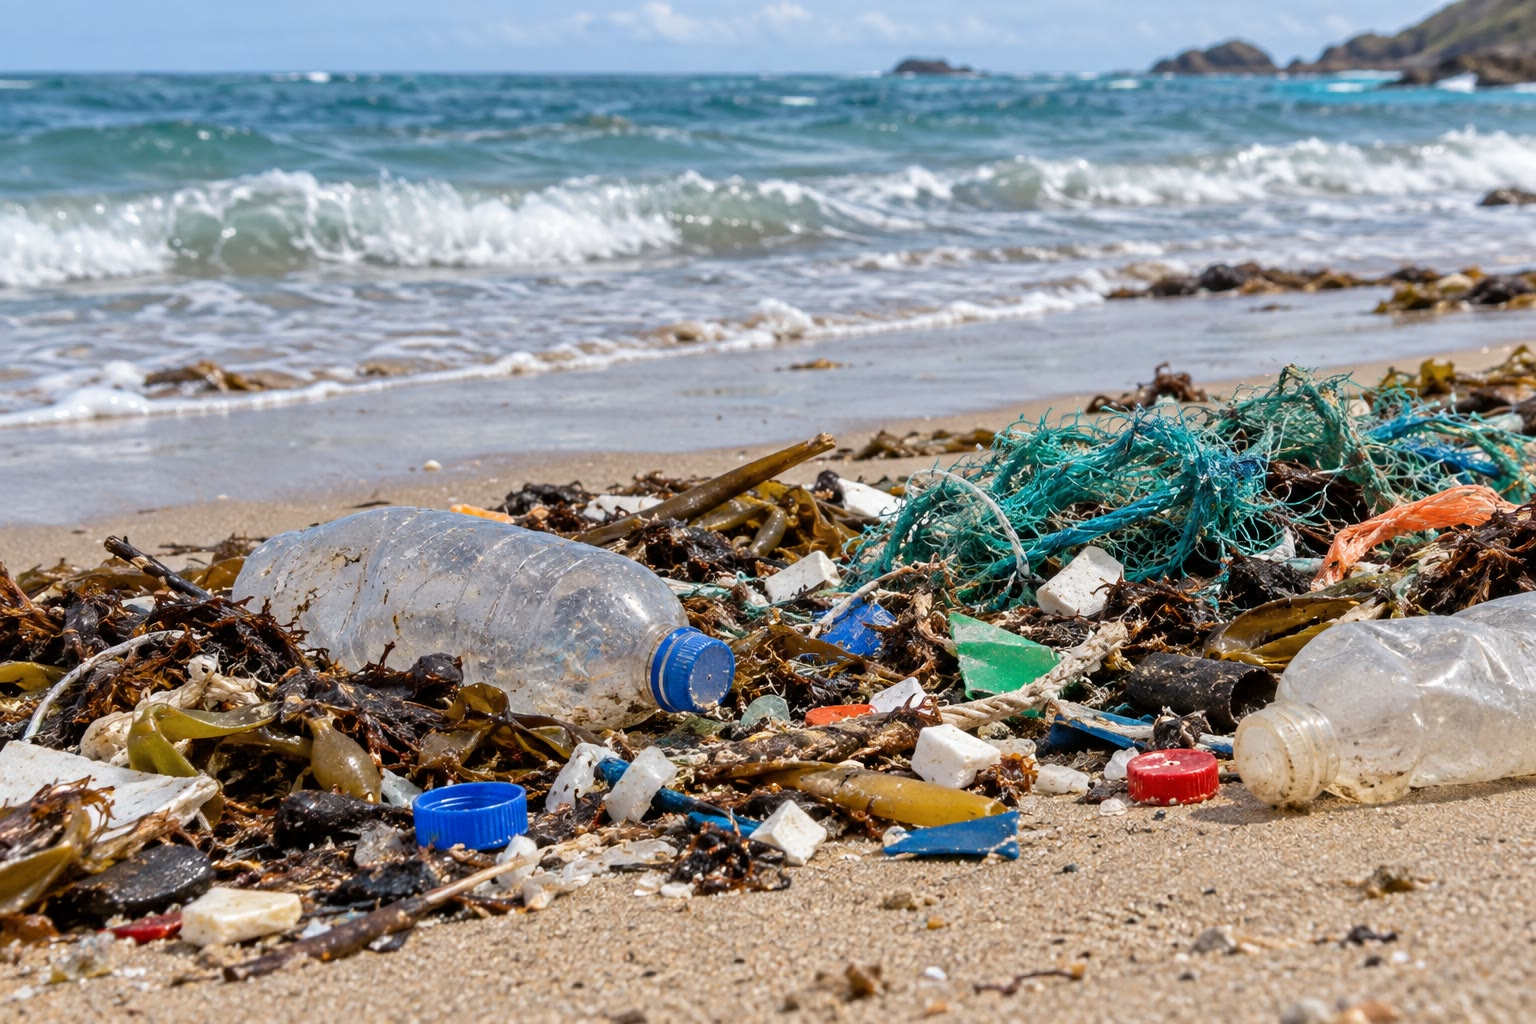
\includegraphics[width=\linewidth,height=4.6cm,keepaspectratio]{images/book1/ai/g8-beach-litter.jpg}

{\small Lixo \omterm{def:g8:plastics:plastic}{plástico} trazido pelo mar até uma praia.}
\end{minipage}\hfill
\begin{minipage}[t]{0.48\linewidth}\centering
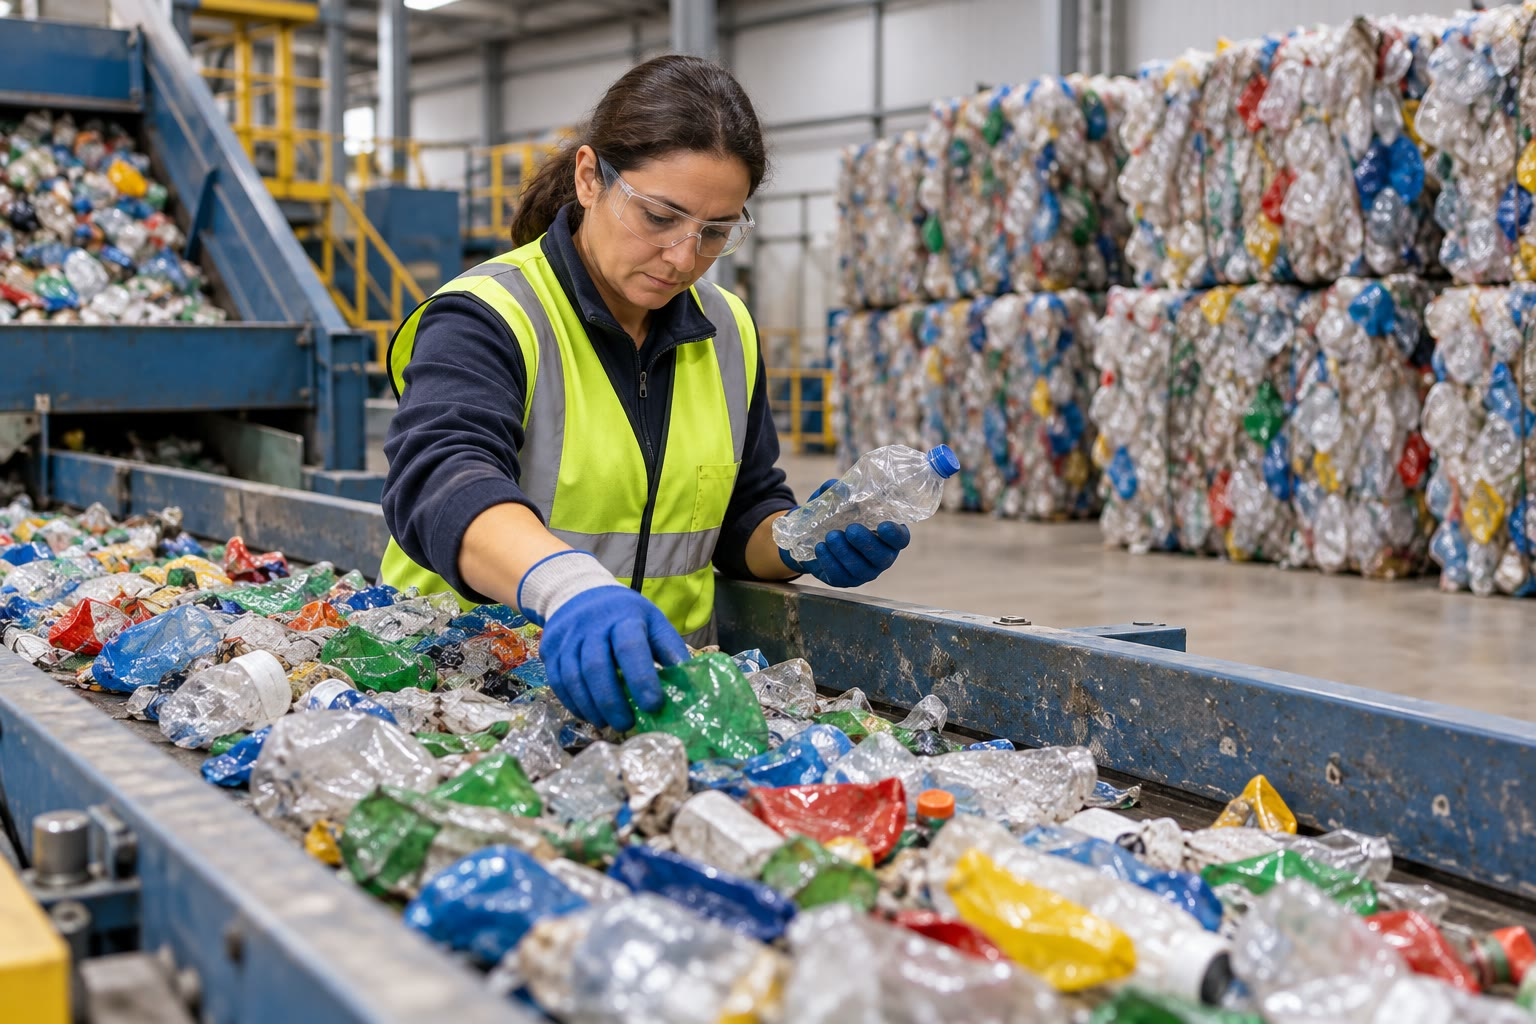
\includegraphics[width=\linewidth,height=4.6cm,keepaspectratio]{images/book1/ai/g8-sorting-line.jpg}

{\small Uma esteira de triagem numa usina de \omterm{def:g5:raw-materials-and-recycling:recycling}{reciclagem} de \omterm{def:g8:plastics:plastic}{plásticos}.}
\end{minipage}
\end{omfigure}

\begin{remark}[Queimar plásticos]\label{rem:g8:plastics:burning}
Os \omterm{def:g8:plastics:plastic}{plásticos} queimam, e fabricam dióxido de carbono quando queimam
completamente. Mas, queimados numa fogueira de quintal, eles queimam de
forma incompleta e liberam fuligem, monóxido de carbono e outras
substâncias nocivas; o PVC, que contém cloro, libera cloreto de
hidrogênio, um gás corrosivo. O lixo \omterm{def:g8:plastics:plastic}{plástico} só é queimado em
incineradores construídos para limpar a fumaça.
\end{remark}

\section{Exercícios}

\begin{exercise}[$\star$]\label{exo:g8:plastics:1}
Natural, artificial ou sintético? Algodão, náilon, papel, lã,
poliestireno, viscose.
\end{exercise}

\begin{exercise}[$\star$]\label{exo:g8:plastics:2}
A partir de que \omterm{def:g5:raw-materials-and-recycling:raw-material}{matéria-prima} a maioria dos \omterm{def:g8:plastics:plastic}{plásticos} é produzida?
\end{exercise}

\begin{exercise}[$\star$]\label{exo:g8:plastics:3}
Que \omterm{def:g8:plastics:plastic}{plástico} tem o código 1? Dê um objeto feito dele.
\end{exercise}

\begin{exercise}[$\star$]\label{exo:g8:plastics:4}
Qual é a diferença entre um \omterm{def:g8:plastics:thermoplastic}{termoplástico} e um \omterm{def:g8:plastics:thermoplastic}{termofixo}?
\end{exercise}

\begin{exercise}[$\star\star$]\label{exo:g8:plastics:5}
Um pote de iogurte traz o código 5. Dê o nome do \omterm{def:g8:plastics:plastic}{plástico} dele, e diga
se, em princípio, ele poderia ser derretido e moldado de novo.
\end{exercise}

\begin{exercise}[$\star\star$]\label{exo:g8:plastics:6}
Por que um triângulo de setas num objeto não quer dizer que o objeto vai
ser reciclado?
\end{exercise}

\begin{exercise}[$\star\star$]\label{exo:g8:plastics:7}
Por que o cabo de uma frigideira muitas vezes é feito de um \omterm{def:g8:plastics:thermoplastic}{termofixo}, e
não de um \omterm{def:g8:plastics:thermoplastic}{termoplástico}?
\end{exercise}

\begin{exercise}[$\star\star$]\label{exo:g8:plastics:8}
Com os números deste capítulo para 2019, que porcentagem do \omterm{def:g8:plastics:plastic}{plástico}
usado virou lixo naquele ano? Arredonde para o número inteiro mais
próximo.
\end{exercise}

\begin{exercise}[$\star\star$]\label{exo:g8:plastics:9}
Por que nunca se deve queimar PVC numa fogueira de quintal?
\end{exercise}

\begin{exercise}[$\star\star$]\label{exo:g8:plastics:10}
Uma escola usa 300 garrafas de \qty{25}{g} cada por semana, durante 36
semanas do ano. Que massa de \omterm{def:g8:plastics:plastic}{plástico} é essa num ano?
\end{exercise}

\begin{exercise}[$\star\star\star$]\label{exo:g8:plastics:11}
O polietileno é formado só por carbono e hidrogênio. Escreva os produtos
da sua \omterm{def:g8:combustion-and-fuels:complete}{combustão completa}. Explique por que queimá-lo acrescenta
dióxido de carbono ao \omterm{def:g4:air-a-mixture-of-gases:air}{ar}, como um \omterm{def:g8:combustion-and-fuels:fossil}{combustível fóssil}.
\end{exercise}

\begin{exercise}[$\star\star\star$]\label{exo:g8:plastics:12}
Explique como uma garrafa de \omterm{def:g8:plastics:plastic}{plástico} perdida no mar pode acabar, anos
depois, como microplásticos dentro de um peixe.
\end{exercise}

\section{Problema: a esteira de triagem}

\begin{problem}[{Problema de fim de semana --- uma tonelada de garrafas
usadas, os códigos delas e os flocos de plástico limpos que saem da
usina}]
\label{pb:g8:plastics:1}
Uma usina de \omterm{def:g5:raw-materials-and-recycling:recycling}{reciclagem} recebe fardos de garrafas de bebida usadas. Um
fardo típico de \qty{1}{t} (\qty{1000}{kg}) contém, em massa:
\qty{80}{\percent} de corpos de garrafa em PET, \qty{12}{\percent} de
tampas (PEAD e PP), \qty{5}{\percent} de rótulos (filme de PP) e
\qty{3}{\percent} de sujeira e restos de líquido. Máquinas separam as
tampas e os rótulos dos corpos, o PET é moído em flocos, e os flocos
são lavados; a lavagem perde \qty{2.5}{\percent} do PET. Os flocos limpos
são derretidos e fiados nas fibras de jaquetas de fleece.

\medskip
\noindent\textbf{Parte I --- Os \omterm{def:g8:plastics:plastic}{plásticos}.}
\begin{enumerate}
  \item Que código está impresso nos corpos das garrafas? E nas tampas?
  \item Esses \omterm{def:g8:plastics:plastic}{plásticos} são naturais, artificiais ou sintéticos?
  \item O PET pode ser derretido e fiado de novo? Que tipo de \omterm{def:g8:plastics:plastic}{plástico}
        isso faz dele?
  \item Por que as tampas e os rótulos são separados dos corpos antes que
        o PET seja derretido?
\end{enumerate}

\medskip
\noindent\textbf{Parte II --- O fardo.}
\begin{enumerate}[resume]
  \item Que massa de PET um fardo contém?
  \item Que massa de tampas? E de rótulos?
  \item Que massa do fardo não é \omterm{def:g8:plastics:plastic}{plástico}?
  \item Que porcentagem do fardo é \omterm{def:g8:plastics:plastic}{plástico}?
\end{enumerate}

\medskip
\noindent\textbf{Parte III --- Os flocos.}
\begin{enumerate}[resume]
  \item Que massa de PET se perde na lavagem?
  \item Uma jaqueta de fleece precisa de \qty{0.39}{kg} de fibra de PET.
        Por que é melhor fabricá-la a partir dos flocos do que a partir
        de PET novo?
  \item A usina poderia queimar as tampas e os rótulos para produzir
        calor em vez de reciclá-los. Dê o nome do gás que isso
        acrescentaria ao \omterm{def:g4:air-a-mixture-of-gases:air}{ar}.
  \item Calcule a massa de flocos de PET limpos que um fardo dá.
\end{enumerate}
\end{problem}
